 
\subsubsection { Общие принципы и введение в алгоритм}

Программирование ограничений — это принципиально иной подход к задаче по сравнению с тремя рассмотренными ранее. Генетический алгоритм, имитация отжига и поиск с запретами — это метаэвристики: они исследуют пространство решений, проверяя сами решения на допустимость постфактум, и не гарантируют ни нахождения наилучшего решения, ни даже корректного определения того, что решения вовсе не существует. Решатель ограничений работает иначе: вместо того чтобы перебирать готовые решения и штрафовать их за нарушения, он описывает задачу как набор переменных с ограниченными областями допустимых значений и набор логических связей между ними, а затем находит значения всех переменных, удовлетворяющие всем связям одновременно, либо строго доказывает, что таких значений не существует. Использованный в данной работе решатель CP-SAT (Constraint Programming — Satisfiability) из состава библиотеки Google OR-Tools объединяет в себе классический аппарат программирования ограничений с современными методами решения задач булевой выполнимости (SAT), что делает его одним из самых быстрых открытых решателей такого класса задач на сегодняшний день.

Принципиальное практическое следствие этого различия — то, как в решателе ограничений реализуются жёсткие ограничения. В трёх предыдущих алгоритмах жёсткое ограничение — это функция, которая после построения кандидата решения проверяет, не нарушено ли оно, и в случае нарушения штрафует решение численно. В CP-SAT жёсткое ограничение, где это возможно, реализуется не как проверка постфактум, а как сужение области допустимых значений переменной заранее: например, переменная «преподаватель данного занятия» с самого начала может принимать только те значения, которые соответствуют преподавателям, действительно квалифицированным по данной дисциплине, — недопустимое значение просто не существует как вариант, и проверять его на допустимость после не требуется.

\subsubsection { Особенности реализации}

Каждое занятие, которое требуется расставить, описывается набором переменных: день недели, номер пары, индекс аудитории внутри заранее отфильтрованного по вместимости и типу списка подходящих аудиторий, и аналогично — индекс преподавателя внутри списка квалифицированных по дисциплине преподавателей. Использование индекса внутри уже отфильтрованного списка, а не прямого идентификатора аудитории или преподавателя, — это и есть тот самый механизм сужения области допустимых значений: недопустимые комбинации физически не входят в эти списки, и решателю не нужно объяснять отдельным правилом, что аудитория должна вмещать группу или что преподаватель должен быть квалифицирован.

Уникальность временного слота занятия — единственное жёсткое ограничение, требующее отдельной явной формулировки, поскольку оно связывает между собой все занятия сразу, а не одно занятие с его собственными параметрами. Для этого день и номер пары каждого занятия объединяются в единый числовой код слота, и накладывается ограничение на то, что все такие коды должны быть попарно различны.

\captionof{listing}{Обьявление всех слотов для предотвращения конфликтов}
\begin{minted}{python}
model.add_all_different([v.slot_id for v in session_vars])
\end{minted}

Любопытное наблюдение, сделанное в процессе формализации модели: ограничение на максимально допустимое число занятий в один день, которое в остальных трёх алгоритмах реализовано отдельной проверяющей функцией, в формулировке через решатель ограничений оказывается автоматическим следствием уже описанного ограничения на уникальность слота в сочетании с тем, что номер пары и так ограничен сверху вместимостью учебного дня: если бы в один день нужно было поставить больше занятий, чем число доступных номеров пар, какие-то два занятия неизбежно получили бы одинаковый номер пары, что само по себе уже запрещено ограничением уникальности. Это пример того, как формальная постановка задачи в виде ограничений иногда вскрывает логические связи между условиями, которые при процедурной, проверочной реализации остаются незамеченными и формулируются как будто бы независимо друг от друга.

Поскольку решатель ограничений требует, чтобы итоговая минимизируемая величина была линейной функцией переменных, один из мягких критериев качества — равномерность загрузки по дням недели, которая в остальных трёх алгоритмах выражена через дисперсию числа занятий по дням, — была заменена на линейный аналог: разницу между максимальной и минимальной загрузкой дня. Это сохраняет содержательный смысл критерия — штраф за неравномерность — но не совпадает с дисперсией число в число, что является осознанным и явно задокументированным отступлением от полной идентичности критериев качества между всеми четырьмя алгоритмами.

\subsubsection { Метрики}

\paragraph{ Стабильность решения при изменении временного бюджета}

Результаты прогонов подтверждают высокую эффективность CP-SAT для размерностей типа medium. Алгоритм доказывает глобальную оптимальность решения в рамках первых 200–210 мс, что делает избыточным выделение значительного временного бюджета.

*Рисунок II.3. Фактическое время работы солвера при различных временных ограничениях*

\begin{figure}[h]
    \centering
    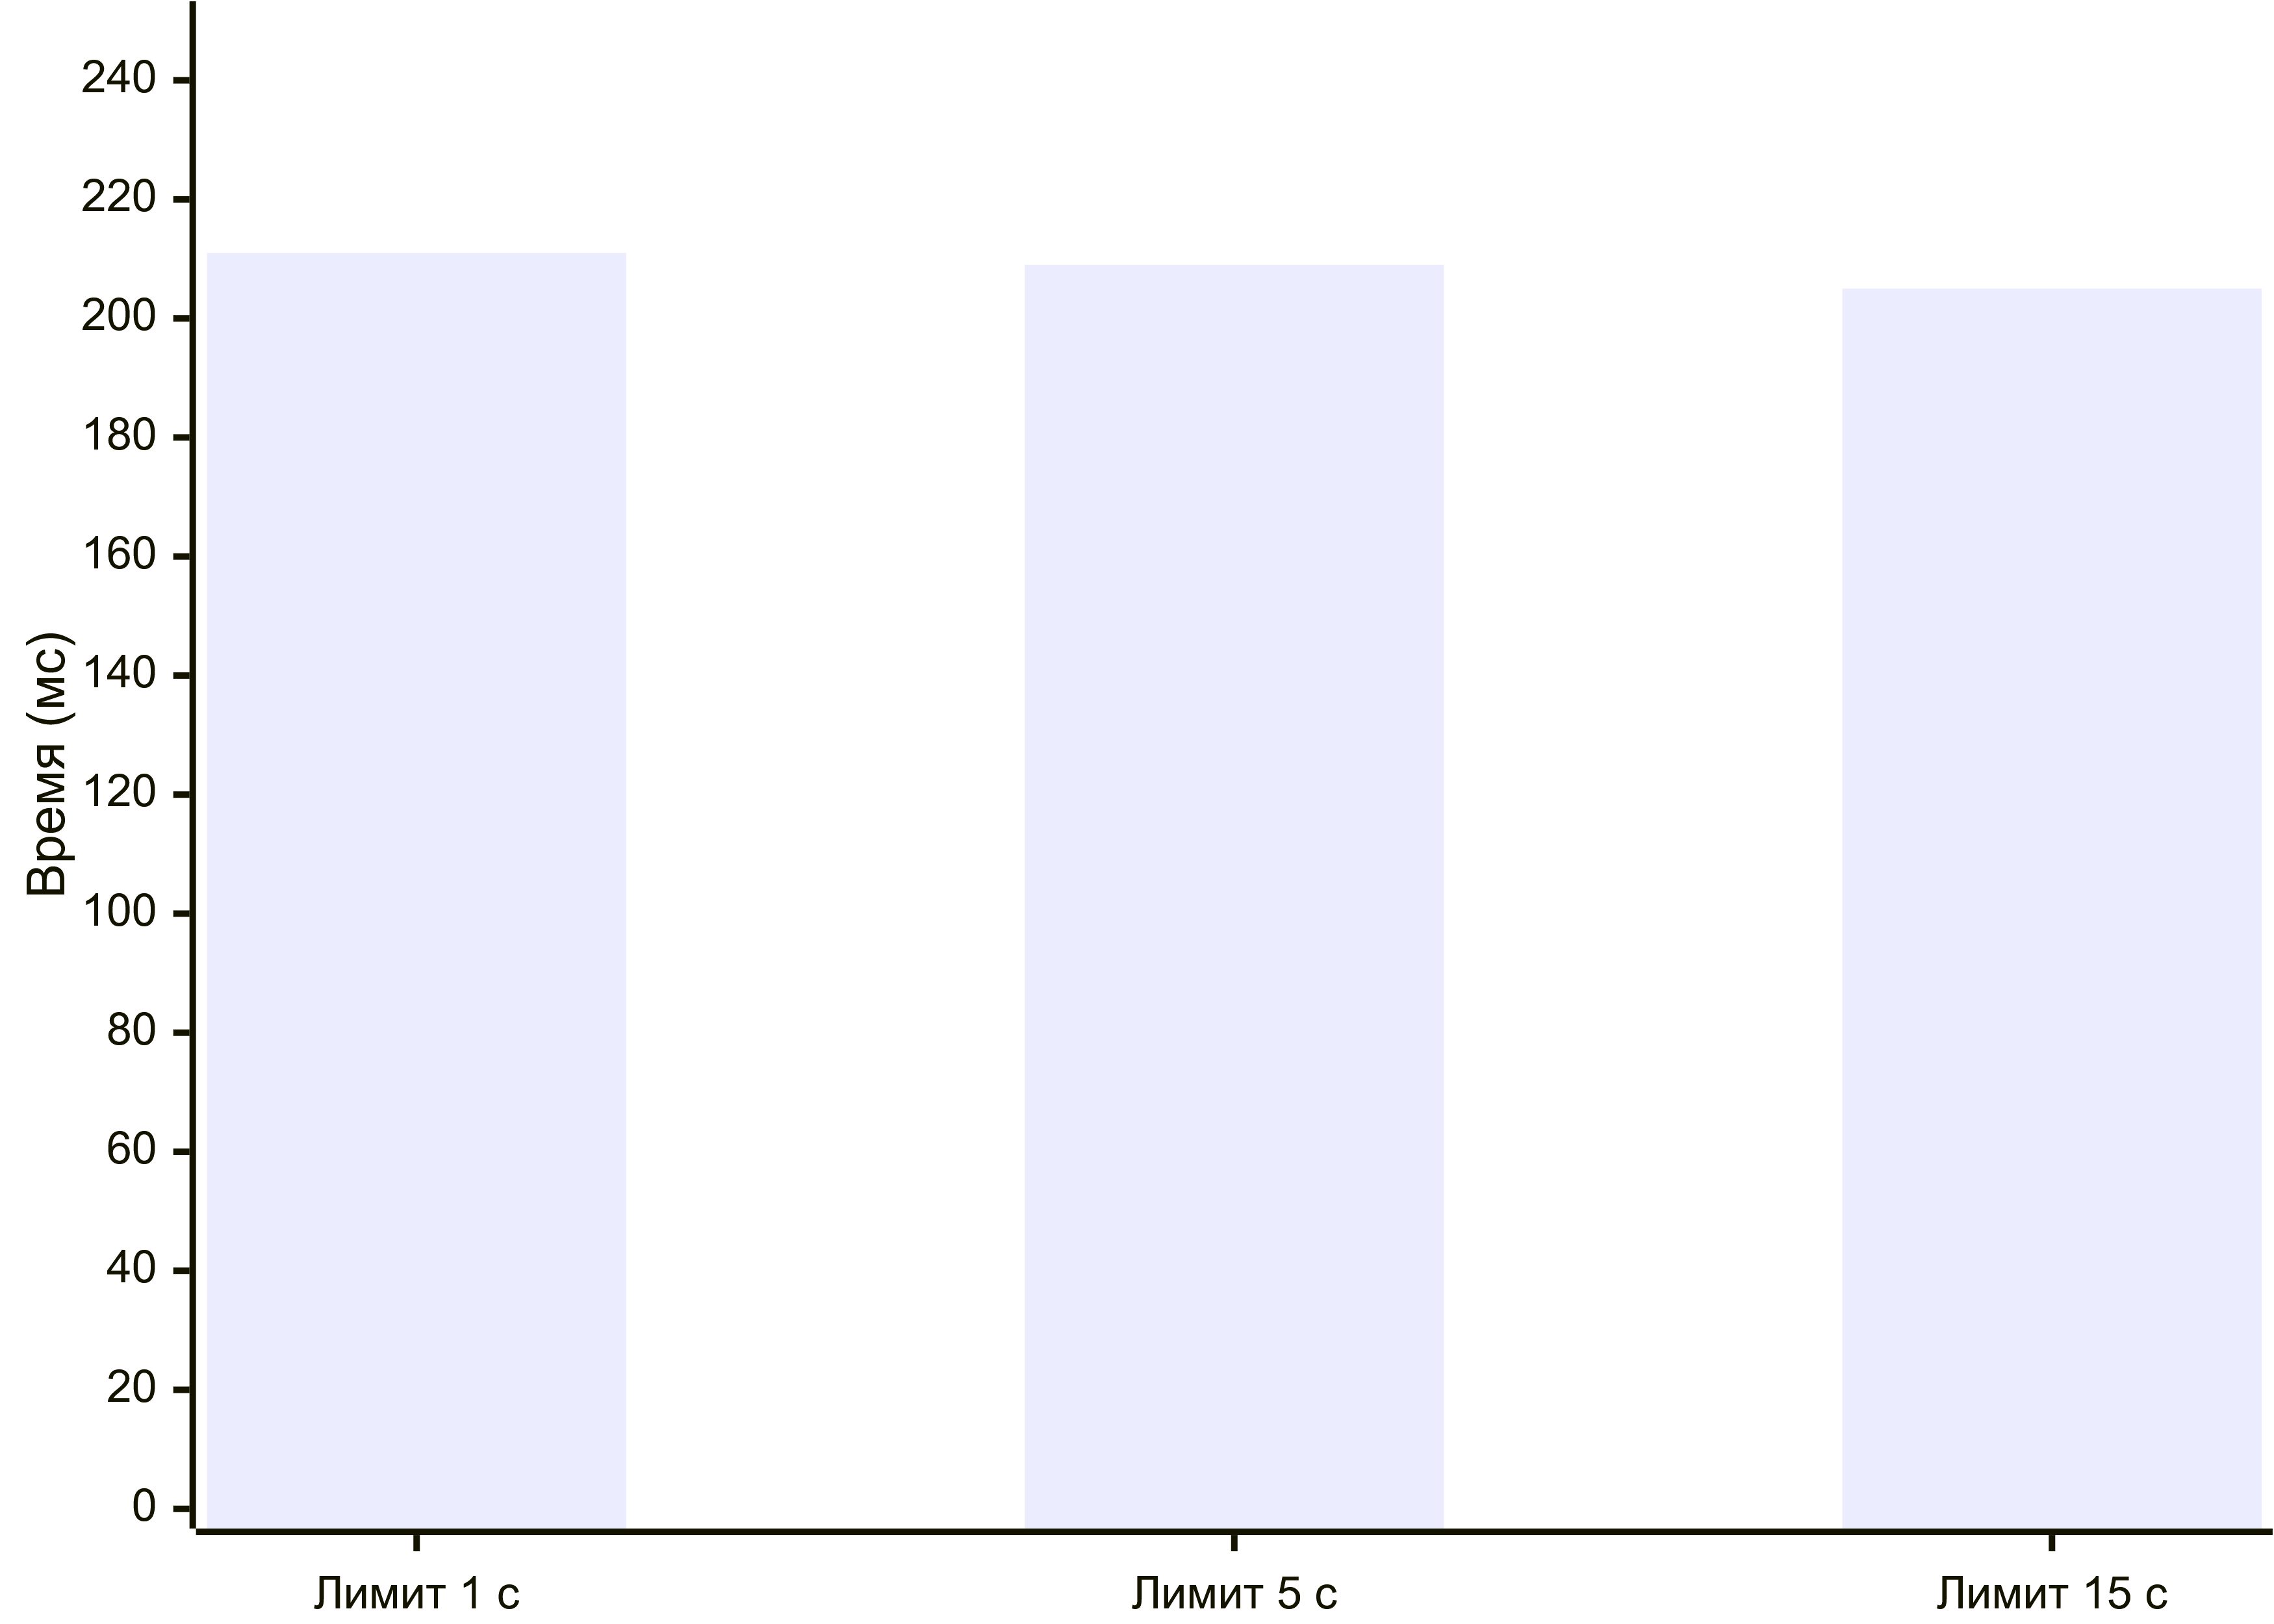
\includegraphics[width=0.8\textwidth]{images/CP Extra Time.png}
    \caption{Фактическое время вычислений при изменении бюджета}
    \label{fig:CPExtraTime}
\end{figure}

\subsubsection { Проблемы, возникшие в процессе реализации}

Основная сложность при формализации модели была связана с вычислением показателя компактности занятий в течение дня — числа «окон» между первым и последним занятием дня. В отличие от трёх остальных алгоритмов, где это вычисляется прямым проходом по уже готовому, полностью определённому расписанию, в решателе ограничений на момент формулировки модели неизвестно, какие именно занятия попадут на какой день — это сама переменная, которую решатель должен подобрать. Потребовалось ввести вспомогательные логические переменные-индикаторы «это занятие стоит в этот день» и связать с их помощью минимальный и максимальный номер пары среди занятий каждого дня, отдельно обработав вырожденный случай дня без единого занятия — без этой отдельной обработки решатель мог бы произвольно манипулировать значениями вспомогательных переменных на пустых днях, искусственно занижая итоговый штраф без какой-либо связи с реальным расписанием.

Корректность итоговой формулировки была дополнительно подтверждена тем, что после нахождения решения оно прогонялось через тот же самый, общий для всех четырёх алгоритмов расчёт количества нарушений жёстких и мягких ограничений: расчёт во всех случаях подтверждал нулевое число жёстких нарушений, что и должно было быть гарантировано самой природой решателя ограничений, а не результатом случайного совпадения.

\subsubsection { Выводы по алгоритму}

Решатель ограничений на всех наборах данных, где допустимое решение существовало, находил решение, доказанно не худшее, чем найденное любым из трёх эвристических алгоритмов, и в большинстве случаев находил его за сопоставимое или меньшее время. На наборе данных, где допустимого решения не существовало вовсе из-за структурного несоответствия между числом занятий и вместимостью учебной сетки, решатель ограничений единственный из всех четырёх алгоритмов дал не просто отрицательный, а доказанный ответ — притом за время, существенно меньшее, чем у любого из эвристических методов, поскольку для доказательства отсутствия решения решателю не требуется производить полноценный поиск по всему пространству вариантов. Это свойство — способность не просто не найти решение, а строго доказать его отсутствие, — оказалось практически значимым и за пределами чисто академического интереса: именно противоречие между ответом решателя ограничений и ответами трёх эвристических алгоритмов на одном и том же наборе данных послужило прямым указанием на дефект реализации, описанный в разделах II.1–II.3.
